\documentclass[10pt,letterpaper]{book}
\usepackage[a4paper,width=15cm,top=2.5cm,bottom=2.5cm,bindingoffset=6mm]{geometry}
\usepackage{footnote}
\usepackage{amsbsy}
\usepackage{amsmath}
\usepackage{physics}
\usepackage{graphicx}
\usepackage{fancyhdr}
\usepackage[T1]{fontenc} % important for having seachable underscores
\usepackage{bm}
\usepackage[sort&compress,numbers]{natbib}
\setlength{\parskip}{2.54mm}


\usepackage{color}
\def\red{\textcolor{red}}
\def\old#1{\textcolor{red}{#1}}
\def\new#1{\textcolor{blue}{#1}}

% Print only chapters in the Table Of Contents
\setcounter{secnumdepth}{2}
\setcounter{tocdepth}{2}

% Ensure that blank pages don't have numbers or heading on them
\makeatletter
\def\cleardoublepage{\clearpage\if@twoside \ifodd\c@page\else
 \hbox{}
 \vspace*{\fill}
 \thispagestyle{empty}
 \newpage\fi\fi}
\makeatother

% set fancy headings
\pagestyle{fancy}
\lhead[{\it \thepage}]{{\bf\it Research Notes}}
\chead{}
\rhead[{\bf\it Research Notes}]{{\it \thepage}}
\renewcommand{\headrulewidth}{0.2pt}
\lfoot{}
\cfoot{}
\rfoot{}
\renewcommand{\footrulewidth}{0pt}
\setlength{\footskip}{0.25in}
\setlength{\parindent}{0in}

%% This part slightly modifies the default definition of \chapter
%% (found in book.cls) to add a \hspace{2em} before numbered chapters.
\makeatletter
\def\@chapter[#1]#2{\ifnum \c@secnumdepth >\m@ne
                       \if@mainmatter
                         \refstepcounter{chapter}%
                         \typeout{\@chapapp\space\thechapter.}%
                         \addcontentsline{toc}{chapter}%
                                   {\hspace{2em}\protect\numberline{\thechapter}#1}%
                       \else
                         \addcontentsline{toc}{chapter}{#1}%
                       \fi
                    \else
                      \addcontentsline{toc}{chapter}{#1}%
                    \fi
                    \chaptermark{#1}%
                    \addtocontents{lof}{\protect\addvspace{10\p@}}%
                    \addtocontents{lot}{\protect\addvspace{10\p@}}%
                    \if@twocolumn
                      \@topnewpage[\@makechapterhead{#2}]%
                    \else
                      \@makechapterhead{#2}%
                      \@afterheading
                    \fi}
\makeatother


% reset vec and hat style to a bold type
\let\oldhat\hat
\renewcommand{\hat}[1]{\oldhat{\mathbf{#1}}}
\renewcommand{\vec}[1]{\mathbf{#1}}
% stretches the vertical spacing of arrays/matrices
\renewcommand{\arraystretch}{2}
\setlength{\jot}{10pt}

\graphicspath{ {./images/} }
\title{Research Notes}
\author{Aidan Winblad}
\date{\today}
%%% THIS SHOULD BE THE LAST PACKAGE TO BE LOADED!
%hidelinks to remove colored borders from links
%plainpages=false needed for the unnumbered pages
%breaklinks=true to allow to break long links (e.g. long titles) on
%more than one line
%bookmarksopen open the bookmarks in the adobe reader plugin
%bookmarksopenlevel decide the max level at which the bookmarks should
%be open
% pdfdisplaydoctitle=true to show the document title instead of the
% filename in the titlebar of adobereader
\usepackage[plainpages=false,breaklinks=true,pdfborder=0 0 0,pdfdisplaydoctitle=true,bookmarksopen=true,bookmarksopenlevel=0,pdftex,%
%Comment next line if it makes problems
%(it requires a recent LaTeX distribution)
            hidelinks,
            pdftitle={MSE502B},
            pdfkeywords={lecture notes}]{hyperref}

\newcommand{\Ham}{\mathcal{H}}


\newcommand{\ke}{k_{\epsilon}}
\newcommand{\kpm}{k_{\pm}}
\newcommand{\sx}{\sigma_x}
\newcommand{\sy}{\sigma_y}
\newcommand{\sz}{\sigma_z}
\newcommand{\so}{\sigma_0}
\begin{document}

\section{Electric Field Limits}

\subsubsection{Dirac}
In the literature quoted in the original FLL draft McIver et al. 10.1038/s41567-019-0698-y they use electric field strengths from $10^7-10^8 V/m$ with $\hbar\omega=191meV$.
They also make a band dispersion graph for a dirac point illuminated by normally incident CPL.
I noticed they are not using the high-frequency (HF) expansion.
Instead, one can build the quasi-energy matrix in momentum space and make a cutoff for the mode then run the eigenvalue solver to get the energy spectrum.
So, I wanted to compare that to the effective Hamiltonian for CPL incident on Dirac cone.
For the HF expansion we require $\hbar \omega \gg \tfrac{v_{F} e E}{2\omega}$ or we can state

\begin{align}
  E &\ll \dfrac{2 \hbar \omega^2}{e v_{F}} \\
  E_{\text{max}} &\approx \dfrac{1}{20} \dfrac{2 \hbar \omega^2}{e v_{F}} \\
  E_{\text{max}} &\approx 3.53 \cdot 10^6 V/m
\end{align}
where I'm assuming a factor of $1/20$ still lets the HF expansion be comparable, $\hbar \omega = 191meV$ and $v_{F} = 1.57 \cdot 10^6 m/s$.
I've plotted the effective energy versus the quasienergy spectrum and they agree fairly well for the given $E_{\text{max}}$.
When using the literature electric field values we get non-matching results

\begin{figure}[h]
  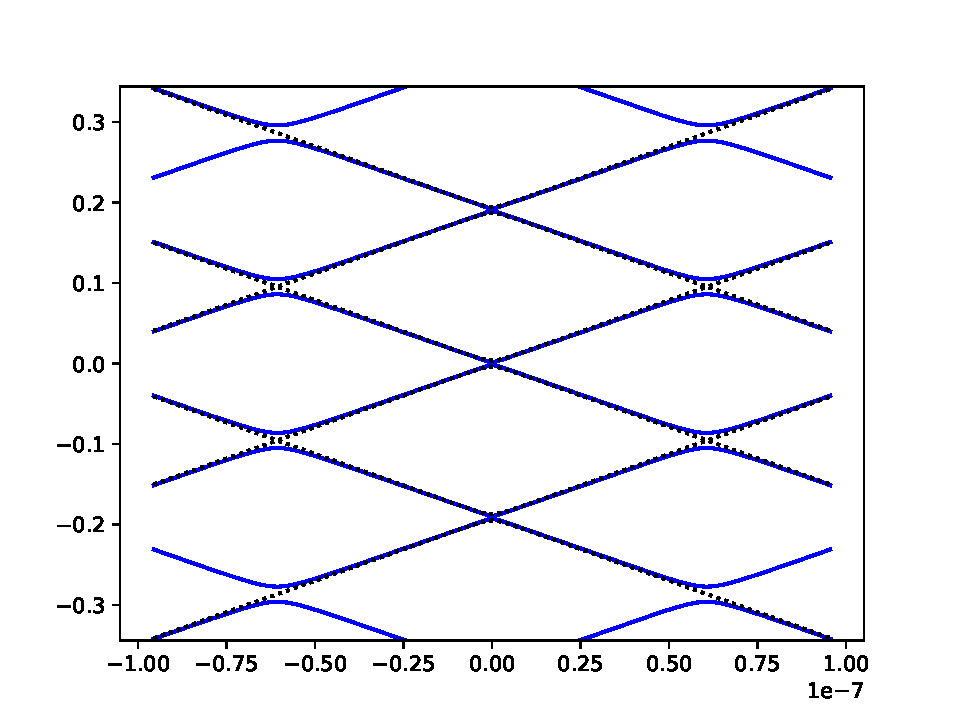
\includegraphics[width=0.33\textwidth]{./energy-spectrum-matching.pdf}
  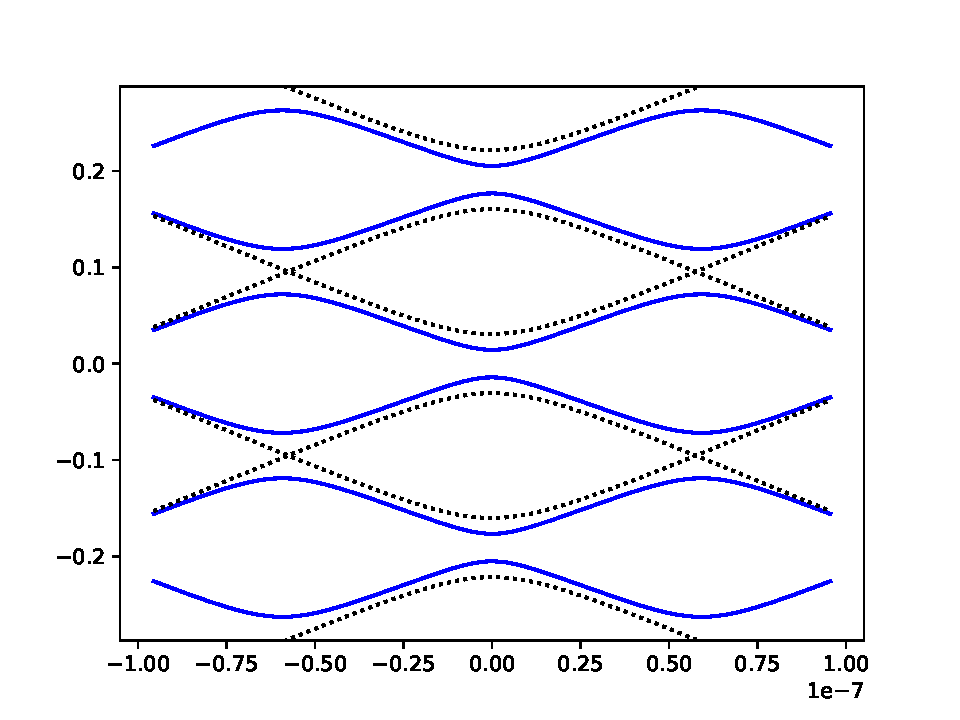
\includegraphics[width=0.33\textwidth]{./energy-spectrum-non-matching.pdf}
  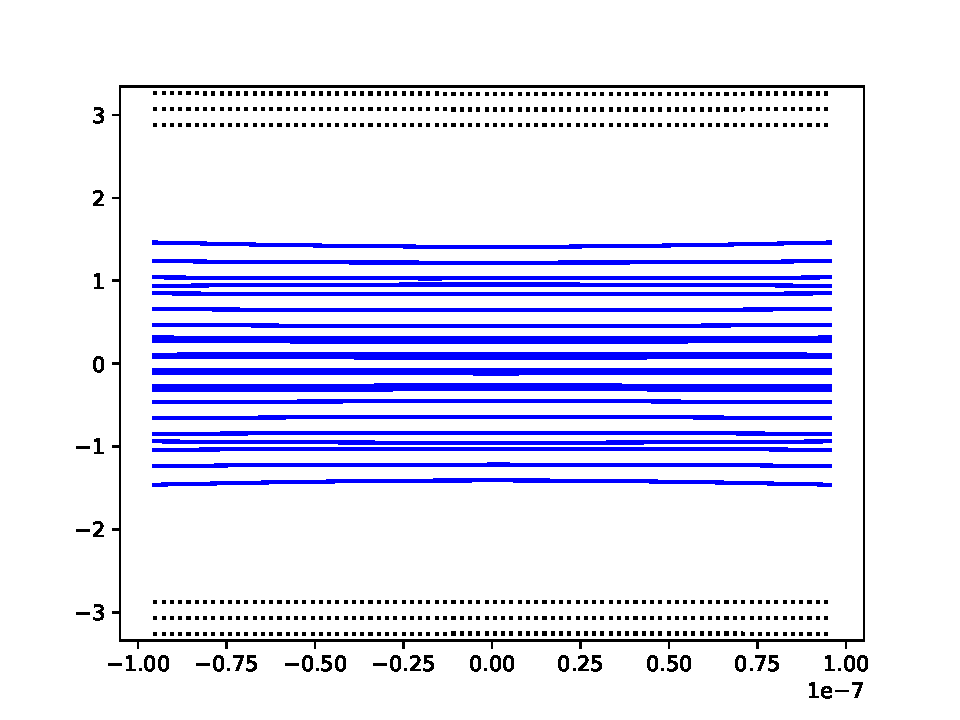
\includegraphics[width=0.33\textwidth]{./energy-spectrum-non-matching-2.pdf}
  \caption{From left to right, $E = 3.53\cdot10^6 V/m$, $E=10^7 V/m$, $E=10^8 V/m$}
\end{figure}
For the given $E_{\text{max}}$ the effective magnetic field is $B_{\text{max}}^D = 1.91 mT$, for $K= 2\pi/d$ with $d=100 nm$.
So we see that $E$ has an upper limit for a given $\hbar \omega$ and $K$ becomes our last tunable parameter, which is also limited by the wavelength with the angle as the last adjustable piece.

\subsubsection{2DEG}

We want to use similar laser parameters for 2DEG, since we know these are easily available in lab.
If we look at the HF expansion fro 2DEG we have a slight alteration, $\hbar \omega \gg |H_{\pm1}| , |H_{\pm2}|$, more explicitly

\begin{align}
  \hbar \omega &\gg \dfrac{eE}{2m^* \omega} \left|\pm ip_x + p_y \cos{(Kx)}\right|, \dfrac{e^2 E^2}{8m^* \omega^2} \sin^2{(Kx)}, \nonumber \\
  \hbar \omega &\gg \dfrac{\hbar eE}{2m^* \omega} k_x , \dfrac{e^2 E^2}{8m^* \omega^2} \sin^2{(Kx)}.
\end{align}
Here I set $k_y=0$, notice that $k_x$ and $x$ are in the expression.
So, I am not sure how to go about this.
Does this mean for smaller values of $k_x$ and $x$ we can make $E$ much larger to allow for the HF expansion?

Let me know what you think about both systems and which values to consider.
Also, the original draft used $\hbar\omega=220meV$ but I could not find that in any of the references cited in that section of the discussion, maybe it is a typo and supposed to be $120meV$?

\end{document}
